\documentclass[12pt]{article}

\usepackage{sbc-template}

\usepackage{graphicx,url}

%\usepackage[brazil]{babel} 
\usepackage[latin1]{inputenc}
\usepackage{nicefrac}
% Change paragraph identation
\setlength{\parindent}{.8cm}
\usepackage{indentfirst}
\newcommand{\etal}{\textit{et. al}}
\usepackage{float}


     
\sloppy

\title{Mineração de dados --- Classificação \\ Análise estatística da base de microdados do ENEM 2012}

\author{Jonathan Coutinho Luz de Queiroz\inst{1} \\ Guilherme Lima Bernal\inst{1}}
\address{Instituto de Matemática -- Universidade Federal da Bahia (UFBA)
\email{jonathanqueiroz@dcc.ufba.br}
}

\newcommand{\reffig}[1]{Fig.~\ref{fig:#1}}
\newcommand{\reftab}[1]{Tabela~\ref{tab:#1}}

\geometry{lmargin=2.2cm, rmargin=2.2cm, tmargin=2.2cm, bmargin=2.2cm}
\setlength\tabcolsep{4pt}
\begin{document} 

\maketitle

\begin{resumo}
Nesta atividade, realizamos uma análise estatística da base de microdados do ENEM 2012, a qual servirá de amparo para o desenvolvimento de um algoritmo de predição da nota de redação.
O primeiro passo consistiu no estudo isolado dos seus principais atributos (idade, sexo, região, localização, tipo de escola e nota de redação).
Em seguida, foi feita uma comparação entre as idades e as notas de redação dos candidatos de cada região do país.
Finalmente, analisamos a correlação entre a nota de redação e diversos outros atributos (idade, sexo, tipo de escola, localização, ano de conclusão do Ensino Médio, notas nas demais provas, deficiência mental e deficiência física).
\end{resumo}

\section{Introdução}
%TODO: especificar "um subconjunto da base"?
Nesta atividade, realizamos uma análise estatística da base de microdados do ENEM 2012.
Como o objetivo final deste trabalho é o desenvolvimento de um algoritmo de predição da nota de redação, o primeiro passo consistiu no descarte de candidatos que não fizeram essa prova (14.672 dentre 50.000).
Em seguida, removemos dois \emph{outliers} de acordo com a idade: um candidato de 7 anos e outro de 114 anos.
Após a remoção desses dois candidatos, a idade passou a variar entre 12 e 70 anos (inclusive), o que indica que os dois registros removidos estão incorretos.
Ainda que não estejam, no entanto, a remoção de dois registros dentre mais de 30.000 é estatisticamente insignificamente e é justificada pela melhoria que isso proporciona na visualização dos gráficos.\footnote{Antes da remoção desses dois registros, mais de $\nicefrac{1}{3}$ da área do histograma de idades era ocupado por valores de 70 a 114, mesmo havendo apenas um registro com valor nessa faixa.}
Restaram 35.326 candidatos.

\section{Estatísticas gerais da base}
\label{sec:estatisticas-gerais}
Antes de iniciarmos uma análise mais aprofundada da base de dados, coletamos algumas estatísticas a respeito dos seus principais atributos, dispostas nos gráficos a seguir.
Conforme evidenciado pela \reffig{candidatos-por-idade}, a maioria dos candidatos possui até 20 anos de idade.
Mais precisamente, dentre os 35.326 candidatos da base, 21.616 (61.2\%) possuem até 20 anos de idade e 28.205 (79.84\%) possuem até 25 anos de idade.
Além disso, como mostra \reffig{candidatos-por-sexo}, há mais candidatos do sexo feminino (59.0\%) do que candidatos do sexo masculino (41.0\%).

\begin{minipage}{.5\textwidth}
    \begin{figure}[H]
    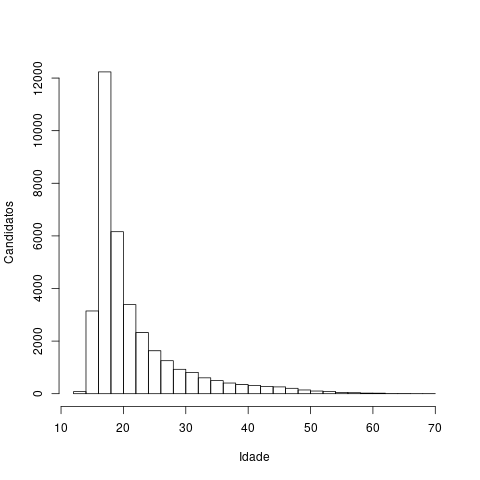
\includegraphics[width=\linewidth]{../geral_candidatos-por-idade.png}
    \caption{Candidatos por idade.}
    \label{fig:candidatos-por-idade}
    \end{figure}
\end{minipage}%
\begin{minipage}{.5\textwidth}
    \begin{figure}[H]
    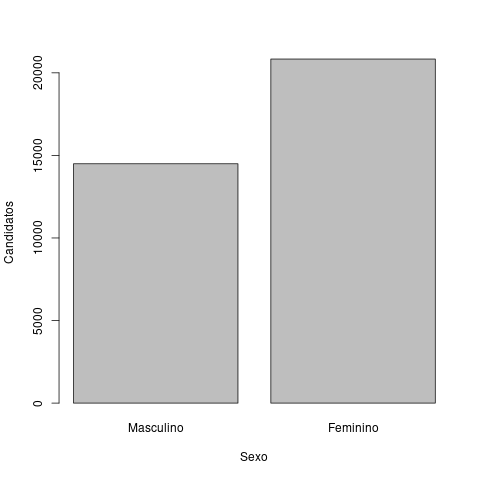
\includegraphics[width=\linewidth]{../geral_candidatos-por-sexo.png}
    \caption{Candidatos por sexo.}
    \label{fig:candidatos-por-sexo}
    \end{figure}
\end{minipage}

Conforme evidenciado pela \reffig{candidatos-por-regiao}, a maioria dos candidatos (68.4\%) está concentrada nas regiões Nordeste e Sudeste.
Além disso, de acordo com a \reffig{candidatos-por-localizacao}, a maioria dos candidatos não informou a localização (zona urbana ou zona rural).
Dentre aqueles que informaram, no entanto, a enorme maioria vive na zona urbana.
\begin{minipage}{.5\textwidth}
    \begin{figure}[H]
    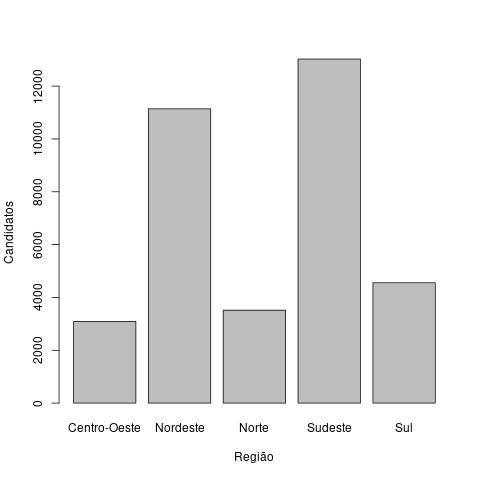
\includegraphics[width=\linewidth]{../geral_candidatos-por-regiao.png}
    \caption{Candidatos por região.}
    \label{fig:candidatos-por-regiao}
    \end{figure}
\end{minipage}%
\begin{minipage}{.5\textwidth}
    \begin{figure}[H]
    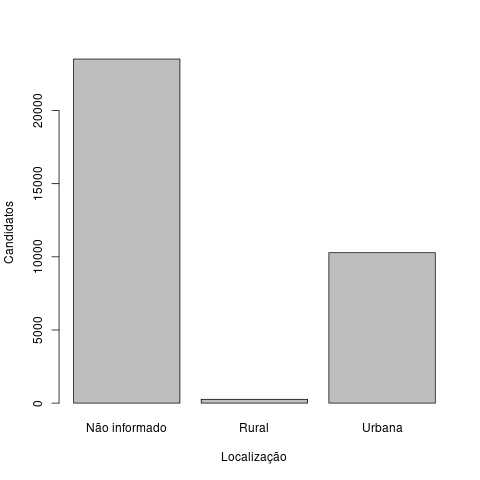
\includegraphics[width=\linewidth]{../geral_candidatos-por-localizacao.png}
    \caption{Candidatos por localização.}
    \label{fig:candidatos-por-localizacao}
    \end{figure}
\end{minipage}


\vspace{1cm}
De acordo com a \reffig{candidatos-por-escola}, a maioria dos candidatos não informou o tipo de escola que frequentou.
Dentre aqueles que informaram, no entanto, a grande maioria estudou em escola pública.
A \reffig{candidatos-por-nota} evidencia a concentração das notas de redação em torno da mediana.
Dos 35.326 canditados, apenas 1507 (4.27\%) obtiveram nota abaixo de 200 e apenas 1.174 (3.32\%) obtiveram nota acima de 800.

\begin{minipage}{.5\textwidth}
    \begin{figure}[H]
    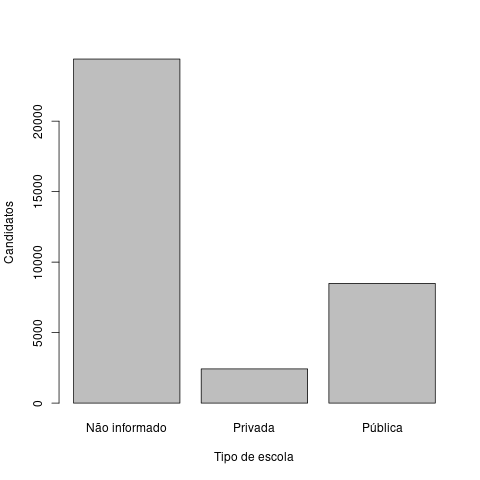
\includegraphics[width=\linewidth]{../geral_candidatos-por-escola.png}
    \caption{Candidatos por tipo de escola.}
    \label{fig:candidatos-por-escola}
    \end{figure}
\end{minipage}%
\begin{minipage}{.5\textwidth}
\begin{figure}[H]
\centering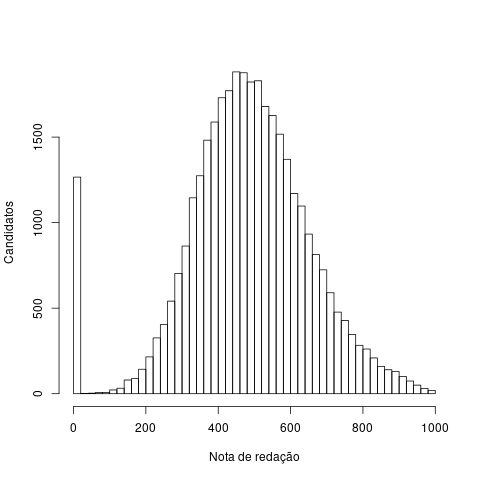
\includegraphics[width=\linewidth]{../geral_candidatos-por-nota.png}
\caption{Candidatos por nota de redação.}
\label{fig:candidatos-por-nota}
\end{figure}
\end{minipage}

\section{Estatísticas por região}
O próximo passo consistiu em gerar estatísticas separadas para cada região, visando a identificação de possíveis associações entre a região do candidado e demais atributos.
Os resultados são apresentados a seguir.

\subsection{Idade}
Conforme evidenciado pela \reftab{idade-por-regiao} e pela \reffig{idade-por-regiao}, a correlação entre a região do candidato e a idade é, em geral, desprezível. Essa correlação se acentua um pouco no caso da região Norte, cujos candidatos tendem a ser, em média, aproximadamente um ano mais velhos, mas ainda assim é pouco significativa.

\begin{minipage}{.5\textwidth}
    \begin{table}[H]
    \begin{tabular}{ c c c c c }
      \textbf{Região}  & \textbf{Candidatos} & \textbf{Média} & \textbf{Mediana} & \textbf{Desvio-padrão} \\
      Brasil           & 35.326              & 22.03          & 19               & 7.48 \\
      Norte            & 3.517               & 22.94          & 20               & 7.52 \\
      Nordeste         & 11.140              & 22.03          & 19               & 7.15 \\
      Sudeste          & 13.024              & 21.69          & 19               & 7.55 \\
      Sul              & 4.555               & 22.01          & 19               & 7.76 \\
      Centro-Oeste     & 3.090               & 22.41          & 19               & 7.81 \\
    \end{tabular}
    \caption{Idade dos candidatos por região.}
    \label{tab:idade-por-regiao}
    \end{table}
\end{minipage}%
\begin{minipage}{.5\textwidth}
    \begin{figure}[H]
    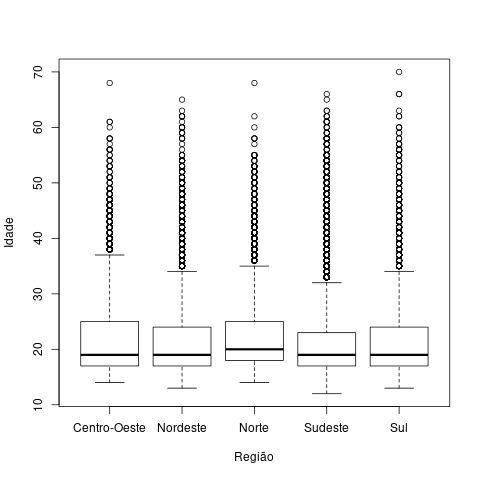
\includegraphics[width=\linewidth]{../regiao_idade.png}
    \caption{Idade dos candidatos por região.}
    \label{fig:idade-por-regiao}
    \end{figure}
\end{minipage}

\subsection{Nota da redação}
A \reftab{nota-por-regiao} e a \reffig{nota-por-regiao} revelam uma leve associação entre a região do candidato e a nota da redação. Mais especificamente, candidatos do Sudesde, e em seguida do Sul, tendem a apresentar notas mais altas que os candidatos das demais regiões. A região com pior desempenho foi a Norte.

\begin{minipage}{.5\textwidth}
    \begin{table}[H]
    \begin{tabular}{ c c c c c }
      \textbf{Região}  & \textbf{Candidatos} & \textbf{Média} & \textbf{Mediana} & \textbf{Desvio-padrão} \\
      Brasil           & 35.326              & 491.49          & 500             & 173.84 \\
      Norte            & 3.517               & 469.24          & 460             & 174.00 \\
      Nordeste         & 11.140              & 478.70          & 480             & 176.39 \\
      Sudeste          & 13.024              & 513.09          & 520             & 172.16 \\
      Sul              & 4.555               & 489.52          & 500             & 169.68 \\
      Centro-Oeste     & 3.090               & 474.77          & 480             & 167.78 \\
    \end{tabular}
    \caption{Nota de redação dos candidatos por região.}
    \label{tab:nota-por-regiao}
    \end{table}
\end{minipage}%
\begin{minipage}{.5\textwidth}
    \begin{figure}[H]
    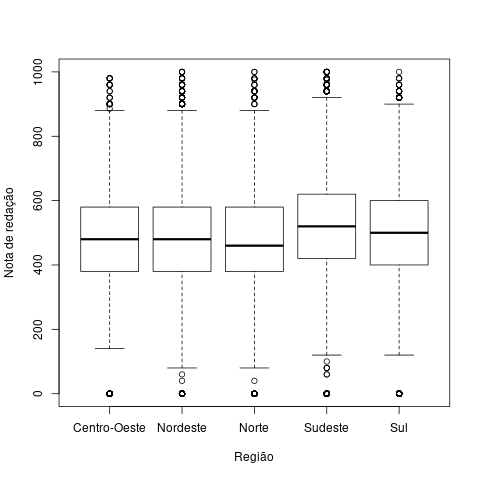
\includegraphics[width=\linewidth]{../regiao_nota.png}
    \caption{Nota de redação dos candidatos por região.}
    \label{fig:nota-por-regiao}
    \end{figure}
\end{minipage}

\section{Análise de correlações}
Finalmente, elegemos alguns atributos para avaliar a existência de possíveis correlações com as notas de redação.
Os resultados são apresentados a seguir.

\subsection{Idade}
%TODO: melhorar essa imagem
A \reffig{correlacao-idade} apresenta as notas de redação em função da idade dos candidatos e aponta para a inexistência de correlação significativa entre esses dois atributos.
De fato, o coeficiente de correlação de Pearson entre essas duas variáveis vale aproximadamente $-0.11$, o que confirma essa hipótese.

\begin{figure}[H]
\centering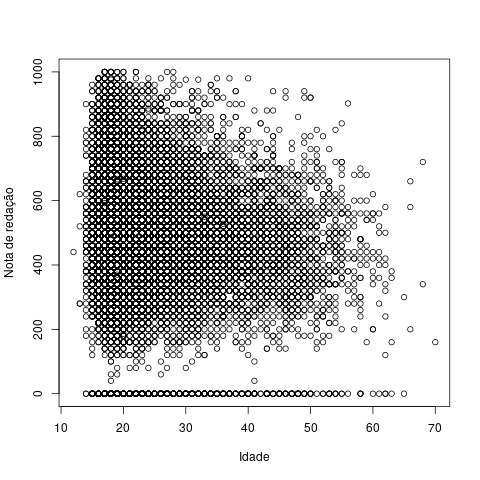
\includegraphics[width=.6\linewidth]{../correlacao_idade.png}
\caption{Notas de redação em função da idade.}
\label{fig:correlacao-idade}
\end{figure}

\subsection{Sexo}
A \reffig{correlacao-sexo} indica que não há diferenças significativas de desempenho entre candidatos do sexo masculino e do sexo feminino.

\begin{figure}[H]
\centering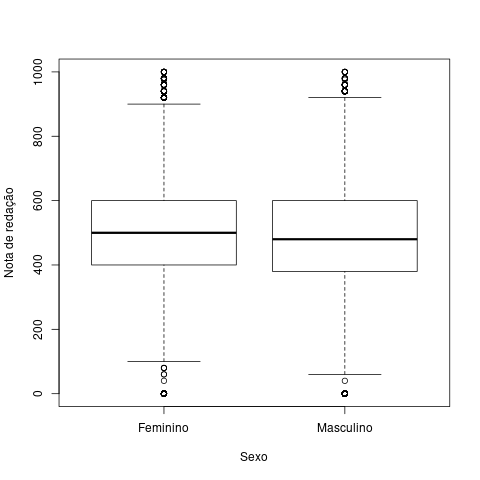
\includegraphics[width=.6\linewidth]{../correlacao_sexo.png}
\caption{Distribuição das notas de redação para candidatos de cada sexo.}
\label{fig:correlacao-sexo}
\end{figure}

\subsection{Tipo de escola}
A \reffig{correlacao-escola} evidencia uma associação entre a nota da redação e o tipo da escola na qual o candidato estudou.
Mais especificamente, estudantes de escolas particulares tendem a obter notas mais altas.
%TODO: ineflizmente, naoad pra usar iso na predicao porque...

\begin{figure}[H]
\centering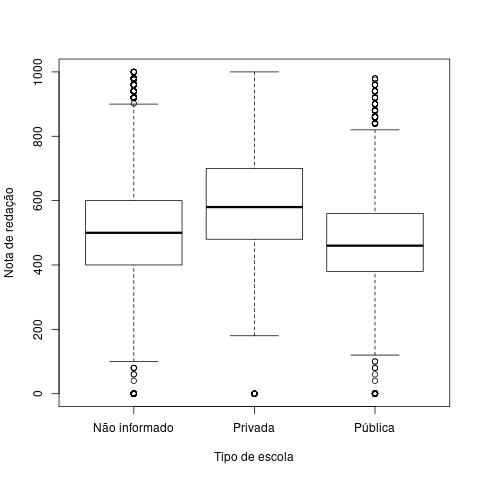
\includegraphics[width=.5\linewidth]{../correlacao_escola.png}
\caption{Distribuição das notas de redação para estudantes de escolas públicas e de escolas privadas.}
\label{fig:correlacao-escola}
\end{figure}

\subsection{Localização}
A \reffig{correlacao-localizacao} evidencia uma associação entre a nota da redação e a localização do candidato (zona urbana ou zona rural).
Mais especificamente, candidatos da zona urbana tendem a obter notas mais altas.
Na seção~\ref{sec:estatisticas-gerais}, mostramos que, dentre os candidatos que informaram a localização, a enorme maioria vive na zona urbana.
A semelhança, na \reffig{correlacao-localizacao}, entre os gráficos dos candidatos que vivem na zona urbana e dos candidatos que não informaram a localização é um possível indício de que a maioria dos candidatos que não informaram localização também vive na zona urbana.

\begin{figure}[H]
\centering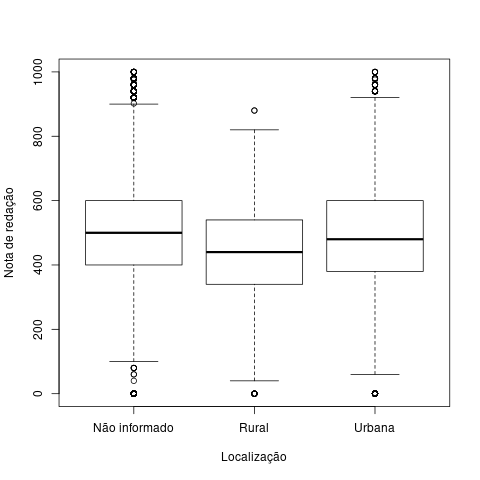
\includegraphics[width=.45\linewidth]{../correlacao_localizacao.png}
\caption{Distribuição das notas de redação para estudantes da zona urbana e da zona rural.}
\label{fig:correlacao-localizacao}
\end{figure}

\subsection{Ano de conclusão do Ensino Médio}
A \reffig{correlacao-ano-concluiu} aponta para a inexistência de correlação significativa entre a nota da redação e o ano no qual o candidato concluiu o Ensino Médio.\footnote{O valor ``.'' indica que o ano de conclusão do Ensino Médio não foi informado.}
\begin{figure}[H]
\centering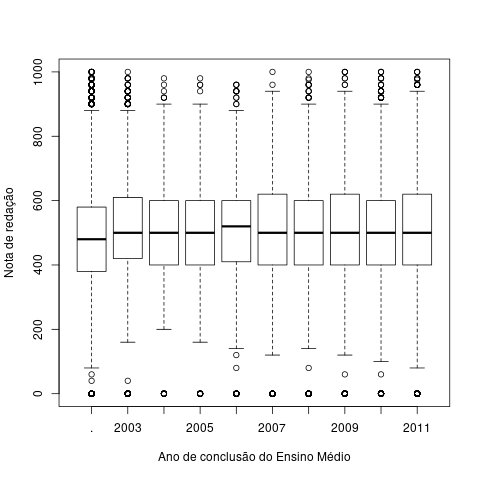
\includegraphics[width=.45\linewidth]{../correlacao_ano_concluiu.png}
\caption{Distribuição das notas de redação em função do ano de conclusão do Ensino Médio.}
\label{fig:correlacao-ano-concluiu}
\end{figure}

\subsection{Notas nas demais provas}
As Figuras~\ref{fig:correlacao-nota-ch}--\ref{fig:correlacao-nota-mt} apresentam uma forte evidência da existência de correlação linear positiva entre as notas obtidas pelos candidatos em redação e nas demais provas.
De fato, os coeficientes de correlação de Pearson apresentados na \reftab{coeficiente-pearson-por-prova} confirmam essa hipótese.
Ainda de acordo com a \reftab{coeficiente-pearson-por-prova}, a maior correlação ocorre com as provas de Ciências Humanas e Linguagens e Códigos.
%TODO: footnote dizendo que foram desconsiderados candidatos que faltaram

\begin{minipage}{.5\textwidth}
    \begin{figure}[H]
    \centering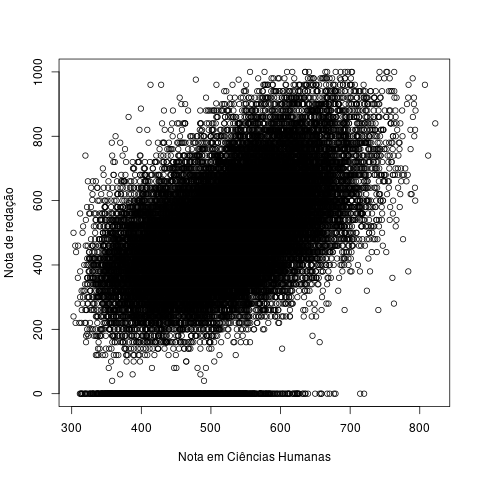
\includegraphics[width=\linewidth]{../correlacao_nota_ch.png}
    \caption{Notas de redação em função das notas em Ciências Humanas.}
    \label{fig:correlacao-nota-ch}
    \end{figure}
\end{minipage}%
\begin{minipage}{.5\textwidth}
    \begin{figure}[H]
    \centering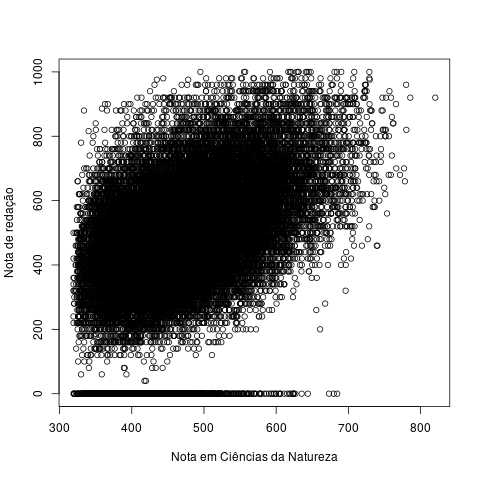
\includegraphics[width=\linewidth]{../correlacao_nota_cn.png}
    \caption{Notas de redação em função das notas em Ciências da Natureza.}
    \label{fig:correlacao-nota-cn}
    \end{figure}
\end{minipage}

\vspace{2cm}

\begin{minipage}{.5\textwidth}
    \begin{figure}[H]
    \centering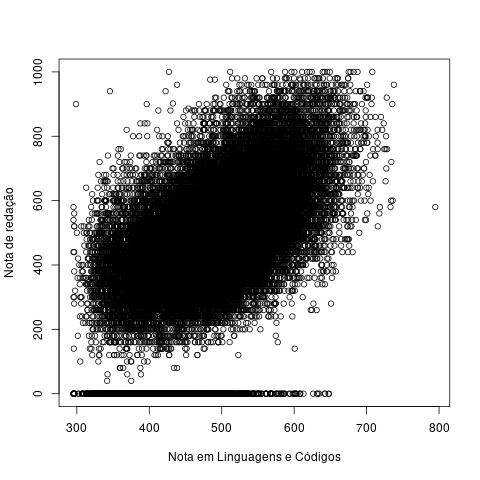
\includegraphics[width=\linewidth]{../correlacao_nota_lc.png}
    \caption{Notas de redação em função das notas em Linguagens e Códigos.}
    \label{fig:correlacao-nota-lc}
    \end{figure}
\end{minipage}%
\begin{minipage}{.5\textwidth}
    \begin{figure}[H]
    \centering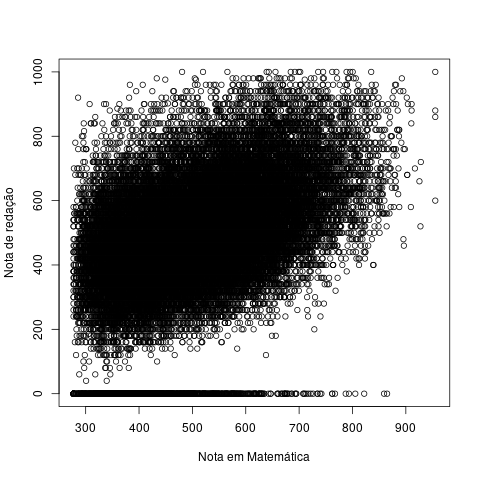
\includegraphics[width=\linewidth]{../correlacao_nota_mt.png}
    \caption{Notas de redação em função das notas em Matemática.}
    \label{fig:correlacao-nota-mt}
    \end{figure}
\end{minipage}

\begin{table}[H]
\centering\begin{tabular}{ c c }
  \textbf{Prova}       & \textbf{Coeficiente de correlação} \\
  Ciências Humanas     & 0.54 \\
  Ciências da Natureza & 0.48 \\
  Linguagens e Códigos & 0.54 \\
  Matemática           & 0.46 \\
\end{tabular}
\caption{Coeficiente de correlação de Pearson entre as notas obtidas pelos candidatos em redação e em cada uma das outras provas.}
\label{tab:coeficiente-pearson-por-prova}
\end{table}

\subsection{Deficiência mental}
A \reffig{correlacao-deficiencia-mental} indica que candidatos com deficiência mental apresentam desempenho significativamente inferior nas provas de redação.

\begin{figure}[H]
\centering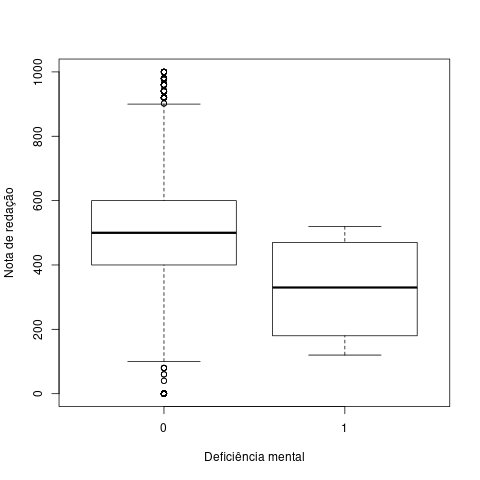
\includegraphics[width=.55\linewidth]{../correlacao_deficiencia_mental.png}
\caption{Distribuição das notas de redação para candidatos com e sem deficiência mental.}
\label{fig:correlacao-deficiencia-mental}
\end{figure}

\subsection{Deficiência física}
A \reffig{correlacao-deficiencia-fisica} indica que a nota mediana de redação dos candidatos com deficiência física é aproximadamente igual à nota mediana de redação dos candidatos sem deficiência física (em torno de 500).
No entanto, a proporção de candidatos com nota acima de 500 é menor para portadores de deficiência física.
\begin{figure}[H]
\centering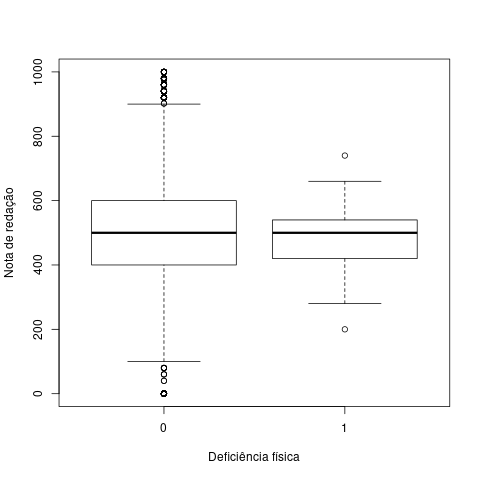
\includegraphics[width=.55\linewidth]{../correlacao_deficiencia_fisica.png}
\caption{Distribuição das notas de redação para candidatos com e sem deficiência física.}
\label{fig:correlacao-deficiencia-fisica}
\end{figure}

\end{document}
